% Options for packages loaded elsewhere
\PassOptionsToPackage{unicode}{hyperref}
\PassOptionsToPackage{hyphens}{url}
%
\documentclass[
  english,
  ,man,floatsintext]{apa6}
\usepackage{lmodern}
\usepackage{amssymb,amsmath}
\usepackage{ifxetex,ifluatex}
\ifnum 0\ifxetex 1\fi\ifluatex 1\fi=0 % if pdftex
  \usepackage[T1]{fontenc}
  \usepackage[utf8]{inputenc}
  \usepackage{textcomp} % provide euro and other symbols
\else % if luatex or xetex
  \usepackage{unicode-math}
  \defaultfontfeatures{Scale=MatchLowercase}
  \defaultfontfeatures[\rmfamily]{Ligatures=TeX,Scale=1}
\fi
% Use upquote if available, for straight quotes in verbatim environments
\IfFileExists{upquote.sty}{\usepackage{upquote}}{}
\IfFileExists{microtype.sty}{% use microtype if available
  \usepackage[]{microtype}
  \UseMicrotypeSet[protrusion]{basicmath} % disable protrusion for tt fonts
}{}
\makeatletter
\@ifundefined{KOMAClassName}{% if non-KOMA class
  \IfFileExists{parskip.sty}{%
    \usepackage{parskip}
  }{% else
    \setlength{\parindent}{0pt}
    \setlength{\parskip}{6pt plus 2pt minus 1pt}}
}{% if KOMA class
  \KOMAoptions{parskip=half}}
\makeatother
\usepackage{xcolor}
\IfFileExists{xurl.sty}{\usepackage{xurl}}{} % add URL line breaks if available
\IfFileExists{bookmark.sty}{\usepackage{bookmark}}{\usepackage{hyperref}}
\hypersetup{
  pdftitle={The Development of Color Terms in Shipibo-Konibo Children},
  pdfauthor={Danielle Kellier*1, Martin Fortier*2, Maria Fernández Flecha3, \& Michael C. Frank4},
  pdflang={en-EN},
  pdfkeywords={keywords},
  hidelinks,
  pdfcreator={LaTeX via pandoc}}
\urlstyle{same} % disable monospaced font for URLs
\usepackage{graphicx,grffile}
\makeatletter
\def\maxwidth{\ifdim\Gin@nat@width>\linewidth\linewidth\else\Gin@nat@width\fi}
\def\maxheight{\ifdim\Gin@nat@height>\textheight\textheight\else\Gin@nat@height\fi}
\makeatother
% Scale images if necessary, so that they will not overflow the page
% margins by default, and it is still possible to overwrite the defaults
% using explicit options in \includegraphics[width, height, ...]{}
\setkeys{Gin}{width=\maxwidth,height=\maxheight,keepaspectratio}
% Set default figure placement to htbp
\makeatletter
\def\fps@figure{htbp}
\makeatother
\setlength{\emergencystretch}{3em} % prevent overfull lines
\providecommand{\tightlist}{%
  \setlength{\itemsep}{0pt}\setlength{\parskip}{0pt}}
\setcounter{secnumdepth}{-\maxdimen} % remove section numbering
% Make \paragraph and \subparagraph free-standing
\ifx\paragraph\undefined\else
  \let\oldparagraph\paragraph
  \renewcommand{\paragraph}[1]{\oldparagraph{#1}\mbox{}}
\fi
\ifx\subparagraph\undefined\else
  \let\oldsubparagraph\subparagraph
  \renewcommand{\subparagraph}[1]{\oldsubparagraph{#1}\mbox{}}
\fi
% Manuscript styling
\usepackage{upgreek}
\captionsetup{font=singlespacing,justification=justified}

% Table formatting
\usepackage{longtable}
\usepackage{lscape}
% \usepackage[counterclockwise]{rotating}   % Landscape page setup for large tables
\usepackage{multirow}		% Table styling
\usepackage{tabularx}		% Control Column width
\usepackage[flushleft]{threeparttable}	% Allows for three part tables with a specified notes section
\usepackage{threeparttablex}            % Lets threeparttable work with longtable

% Create new environments so endfloat can handle them
% \newenvironment{ltable}
%   {\begin{landscape}\begin{center}\begin{threeparttable}}
%   {\end{threeparttable}\end{center}\end{landscape}}
\newenvironment{lltable}{\begin{landscape}\begin{center}\begin{ThreePartTable}}{\end{ThreePartTable}\end{center}\end{landscape}}

% Enables adjusting longtable caption width to table width
% Solution found at http://golatex.de/longtable-mit-caption-so-breit-wie-die-tabelle-t15767.html
\makeatletter
\newcommand\LastLTentrywidth{1em}
\newlength\longtablewidth
\setlength{\longtablewidth}{1in}
\newcommand{\getlongtablewidth}{\begingroup \ifcsname LT@\roman{LT@tables}\endcsname \global\longtablewidth=0pt \renewcommand{\LT@entry}[2]{\global\advance\longtablewidth by ##2\relax\gdef\LastLTentrywidth{##2}}\@nameuse{LT@\roman{LT@tables}} \fi \endgroup}

% \setlength{\parindent}{0.5in}
% \setlength{\parskip}{0pt plus 0pt minus 0pt}

% \usepackage{etoolbox}
\makeatletter
\patchcmd{\HyOrg@maketitle}
  {\section{\normalfont\normalsize\abstractname}}
  {\section*{\normalfont\normalsize\abstractname}}
  {}{\typeout{Failed to patch abstract.}}
\patchcmd{\HyOrg@maketitle}
  {\section{\protect\normalfont{\@title}}}
  {\section*{\protect\normalfont{\@title}}}
  {}{\typeout{Failed to patch title.}}
\makeatother
\shorttitle{Color Terms in Shipibo-Konibo Children}
\keywords{keywords\newline\indent Word count: X}
\usepackage{lineno}

\linenumbers
\usepackage{csquotes}
\ifxetex
  % Load polyglossia as late as possible: uses bidi with RTL langages (e.g. Hebrew, Arabic)
  \usepackage{polyglossia}
  \setmainlanguage[]{english}
\else
  \usepackage[shorthands=off,main=english]{babel}
\fi

\title{The Development of Color Terms in Shipibo-Konibo Children}
\author{Danielle Kellier*\textsuperscript{1}, Martin Fortier*\textsuperscript{2}, Maria Fernández Flecha\textsuperscript{3}, \& Michael C. Frank\textsuperscript{4}}
\date{}


\affiliation{\vspace{0.5cm}\textsuperscript{1} University of Pennsylvania\\\textsuperscript{2} PSL Research University\\\textsuperscript{3} Pontificia Universidad Católica del Perú\\\textsuperscript{4} Stanford University}

\abstract{
Enter abstract here. Each new line herein must be indented, like this line.
}



\begin{document}
\maketitle

TO BE PASTED FROM GOOGLE DOC

\hypertarget{introduction}{%
\section{Introduction}\label{introduction}}

Color language is where language and perception meet. Terms like \emph{blue} or \emph{red} draw boundary lines across a perceptually continuous space. In English, there are 11 basic color terms, but this color categorization is not universal. For instance, Russian speakers use two distinct words to describe the colors light blue (\enquote{goluboy}) and dark blue (\enquote{siniy}); and some languages have as few as two words (e.g., the Jalé people only have terms for ``light'' and ``dark''; Berlin \& Kay, 1969). Why do languages vary in their color systems? One emerging consensus is that languages categorize the color spectrum in different ways in part due to functional demands (Gibson et al., 2017): both smaller and larger color systems are relatively optimal for suiting different communicative needs (Regier, Kay, \& Khetarpal, 2007).

One important component of this hypothesis is the idea that some color systems are easier to learn for children than others; but the actual acquisition of color terms -- while well-studied in English (e.g., Wagner, Dobkins, \& Barner, 2013) -- is extremely under-studied across other populations. Berlin \& Kay's seminal World Color Survey (WCS; Kay, Berlin, Maffin, Merrifield, \& Cook, 2009) presented adult speakers of over 100 languages with differently colored chips and asked them to produce a label, characterizing the space of color vocabulary in a range of written and unwritten languages. The WCS is an invaluable resource for the cross-linguistic study of color vocabulary, but no comparable resource exists for cross-cultural studies of how this vocabulary is learned across childhood.

In the current project, our goals were (1) to characterize color term knowledge in an indigenous population previously studied by the WCS, the Shipibo-Konibo (SK), and then (2) to build on this foundation to characterize the developmental trajectory of color language acquisition in a group of children raised outside of the WEIRD (Western Educated Industrialized Rich Democratic) populations that are over-represented in behavioral science.

\hypertarget{color-in-amazonian-languages-and-latin-american-varieties-of-spanish}{%
\subsection{Color in Amazonian languages and Latin American varieties of Spanish}\label{color-in-amazonian-languages-and-latin-american-varieties-of-spanish}}

A few studies explore the use of color terms in the varieties of Spanish in Latin America. Berlin and Kay (1969) examine the case of the Mexican dialect of Spanish, which they consider to be in Stage VII of their classification. So, for example, a Stage II system would add the term red to the colors already present in Stage I (\emph{black} and \emph{white}). It wouldn't be possible for a system to have \emph{red} if it doesn't already have \emph{black} and \emph{white}. They identify the following basic color terms: \emph{blanco} (white), \emph{negro} (black), \emph{rojo} (red), \emph{verde} (green), \emph{amarillo} (yellow), \emph{azul} (blue), \emph{café} (brown), \emph{morado} (purple), \emph{rosa} (pink), \emph{anaranjado} (orange) and \emph{gris} (grey). Also, based on their work with forty Tzeltal participants, both Tzeltal monolinguals as well as Tzeltal-Spanish bilinguals, they found that bilingualism did not skew their results regarding the existence of semantic universals in the domain of color vocabulary. Tzeltal has five basic color terms: \emph{?ihk´} (black), \emph{sak} (white), \emph{cah} (red), \emph{yaš} (green) and \emph{k´an} (yellow). This language is estimated to be transitioning from Stage IV to V, which is reflected in the ambiguity of the focus of \emph{yaš} (grue). The authors posit that a long history of contact with Spanish has probably accentuated this, and suggest that exposure to Spanish in schools will eventually cause \emph{yaš} to be entirely restricted to greens, and \emph{azul} (or some other Spanish term) will be adopted into the Tzeltal color system.

Monroy and Custodio (1989) offers information on Colombian Spanish based on materials collected for the Linguistic-ethnographic Atlas of Colombia. He presents examples of ad hoc color terms referring to colors through objects prototypically instantiating these color: \enquote{vegetables}, \enquote{animals}, \enquote{food}, \enquote{metals}, \enquote{precious stones}, \enquote{fire and its derivatives} and \enquote{atmospheric phenomena}.

More recently, Aragón (2016) offers an ethnolinguistic study of color terms in Mexican Spanish: \emph{amarillo} (yellow), \emph{azul} (blue), \emph{blanco} (white), \emph{café} (literally \enquote{coffee}, but effectively brown), \emph{gris} (gray), \emph{morado} (purple), \emph{naranja} (orange), \emph{negro} (black), \emph{rojo} (red), \emph{rosado} (pink) and \emph{verde} (green). She analyzes the elaboration of these meanings in dictionaries, as well as the references and associations to which informants resort to for their own definitions. Aragón concludes that the local natural and cultural referents constitute a point of consensus among Mexicans when defining terms of color. Although informants also discussed some cultural material referents, these were not salient prototypes in their explanations. A special case that would merit further study in the future is that of \emph{café} in Mexico versus \emph{marrón} in Spain. According to the author, these two color terms are differentiated by the prototype \enquote{toasted coffee grain} associated to the Mexican Spanish term. Finally, she reviews the symbolic associations related to some terms, such as the discourses on femininity, especially those centered around the figure of the girl, associated with the term \emph{rosado.}

Gibson et al. (2017) offer some approximations to the case of color terms in Bolivian Spanish, based on their analysis centered on Tsimane, an indigenous language spoken by a group living in the Amazonian piedmont. The authors compare the Tsimane case with Bolivian Spanish and American English. Compared to Bolivian Spanish and English, Tsimane exhibits greater variability in terms of the color terms used for all color chips presented in their study, with the exception of red. Out of a total of 80 color chips, Tsimane exhibits 8 modal color terms while English has 10, and Bolivian Spanish, 11. Also, despite the variability observed, the assignment of modal color terms resulted in a similar partition of the color space in the three languages assessed. The authors also emphasize that the Tsimane color system is less informative than the English and the Bolivian Spanish one. Finally, using the free choice paradigm, they show speakers of Bolivian Spanish extensively use the term \emph{verde} (green) to denominate the color chips displayed, in addition to \emph{celeste} (light-blue) and \emph{azul} (blue), as well as \emph{morado} (purple). Less frequent terms are, for example, \emph{fucsia} (fuchsia), \emph{guinda} (maroon) and \emph{mostaza} (mustard).

Several indigenous Amazonian color systems have been studied in the WCS. One of them, Candoshi, has been further examined by Surrallés (2016). In this thought-provoking study, Surrallés suggests that no proper color term exists in this language. If the fieldworkers of the WCS found otherwise, it is only because they misidentified the elicited terms as color terms while they are nothing more than a series of ad hoc terms referring to objects or animals of the surrounding environment. For example, in Candoshi, the word for yellow is \enquote{\emph{ptsiyaromashi}} (\enquote{like the feathers of a milvago bird}), the word for red is \enquote{\emph{chobiapi}} (\enquote{ripe fruit}), the word for green is \enquote{\emph{kamachpa}} (\enquote{unripe fruit}), etc. These findings lead Surrallés to argue that the Candoshi do not have a proper color system. When they use \enquote{color terms} they are not trying to subsume objects of the world under abstract color categories, but they are rather establishing horizontal and ad hoc comparisons between similar objects of the world.

A similar criticism of the WCS approach had been previously developed by Everett (2005, pp. 627--628) based on his study of Pirahã, another Amazonian language. Everett also rejects the idea that there are basic color terms in this language. He argues that the four color terms identified as basic in the WCS are not such. For example, the word identified as the basic color term for \enquote{red} and \enquote{yellow} (\emph{bi i sai}) means nothing more than \enquote{bloodlike}. Here again, color terms seem to be ad hoc comparisons rather than proper basic terms.

As mentioned earlier, SK color terms have been thoroughly studied in the WCS. It is worth mentioning that two anthropological studies (Morin, 1973; Tournon, 2002) have also investigated the color terms used in this Amazonian language. However, these two studies contain some serious methodological pitfalls: a very limited number of chips were tested with only a few participants. As a result, we will not further discuss these studies in the remaining of this article and will only focus on a comparison with the WCS data.

In sum, while some dialectical differences can be noticed across varieties of Spanish, these slight variations are consistent with the general framework proposed by the WCS. Less consistent, however, is the recurrent finding that ad hoc terms seem to play a central role in Amazonian color systems -- and possibly also in some South-American varieties of Spanish (such as Colombian Spanish). More broadly, it seems that Amazonian color systems are characterized by fewer color terms than dialectical Spanish systems.

\hypertarget{the-development-of-color-vocabulary}{%
\subsection{The Development of Color Vocabulary}\label{the-development-of-color-vocabulary}}

\hypertarget{the-current-study}{%
\subsection{The Current Study}\label{the-current-study}}

In the last two decades, cross-cultural research aiming to go beyond North-American \enquote{convenience samples} has mainly focused on the study of East Asian children and adults. This endeavor has proved very fruitful (Kitayama \& Cohen, 2007) but is still limited because of its almost exclusive focus on North-American vs.~East-Asian samples. The current study contributes to the general effort to go beyond such samples and study the development of human cognition in a non-North American and non-East Asian context.
The SK people are an indigenous group located within the Peruvian Amazon. They are mainly horticulturalists, fishermen, occasionally hunters but are noted for their strong display of tradition despite increasingly regular interactions with the western world. Their children receive formal schooling for 4 hours a day and begin formal Spanish lessons closer to adolescence. Most SK adults have some grasp of Spanish but younger adults show more proficiency than elders.

The SK indigenous people are particularly interesting for at least two reasons:
They differ from samples usually studied by cross-cultural evolutionary psychologists (Apicella \& Barrett, 2016). Indeed, evolutionary psychologists are particularly interested in the study of contemporary hunter-gatherers because they are believed to be a good model of our Pleistocene ancestors. By contrast, like most riverine Amazonian cultures, the SK culture is not based on hunting and gathering, but on horticulture, fishing, and to a limited extent, hunting.

Because of their location on the Ucayali River, one of the main tributaries of the Amazon, the SK culture has always been enmeshed in rich trading networks involving other indigenous groups of the Andes and the Lowlands (in pre-conquest times) as well as Mestizos and Westerners (in post-conquest times) (Lathrap, 1970). It would thus be mistaken to think of this culture as an \enquote{isolated} or \enquote{preserved} one. On the contrary, having been extensively exposed to numerous cultural influences, the SK culture has been constantly reworked and reshaped through the centuries. This was especially true in the second half of the 20th century with intense contact with the Spanish-speaking Mestizo populations established along the Ucayali River. As a result, today's SK culture straddles two worlds.

\hypertarget{study-1}{%
\section{Study 1}\label{study-1}}

Before we could assess the developmental trajectory of color term knowledge in SK children, our goal was to replicate and update the characterization of the adult SK color system given by the World Color Survey. As the WCS study took place generations prior, we could not assume the SK color term mappings had remained static especially through years of industrialization and exposure to the Spanish language and its own color term system. As such, Study 1 served as a modified version of the original WCS protocol, down to use of an identical chip set, in order to generate a standard against which subsequent child participants could be scored.

\hypertarget{methods}{%
\subsection{Methods}\label{methods}}

\hypertarget{participants}{%
\subsubsection{Participants}\label{participants}}

Our protocol for Study 1 and all subsequent studies received ethical approval from Pontificia Universidad Católica del Perú's Institutional Review Board. We recruited 39 adult participants (7 men). We experienced difficulty recruiting male participants as many of the men were away from the village during the day, resulting in a sample that is predominantly female. Most participants (31, 4 men) were from SK communities of the Middle Ucayali region (Yarinacocha, San Francisco, and Nueva Betania), with a subset from communities of the Lower (Paoyhan) and Upper (Puerto Belén) Ucayali region. Within the small town of Yarinacocha (in the vicinity of Pucallpa), we recruited participants (9, 2 men) from the predominantly SK neighborhood of Bena Jema. All the other recruitment sites were native community villages with exclusively SK residents. Overall, the sample included SK adults who could be characterized as more urban (Yarinacocha and San Francisco sites) or more traditional and in regular contact with the surrounding rainforest (Nueva Betania, Paoyhan, and Puerto Belén sites).

The median age for participants was 38 years (\emph{IQR} = 26-48 years) ranging from 20 to 64 years. Regarding occupations, 13 of the 32 female participants were homemakers or housewives (33\% of the overall sample) and another 13 were artisans (33\%). Three of the 7 male participants (8\% overall) were horticulturalists. Across both sexes, 5 women and 3 men identified as students, comprising a total 21\% of the population. Although all adult participants were required to be native SK speakers, all but 1 participant had been introduced to the Spanish language prior to adolescence (median age = 8yo, \emph{IQR} = 5-10). Participant age and reported age of introduction to Spanish were positively correlated; younger participants reported learning Spanish at an earlier age (\emph{r} = \(t(35) = 2.81\), \(p = .008\)).

\hypertarget{materials-and-procedure}{%
\subsubsection{Materials and procedure}\label{materials-and-procedure}}

Similar to the original WCS, we used an identical set of 330 color chips but with notable changes in procedure. In the WCS, every participant provided terms for all 330 chips. Due to fear of participant fatigue, we split up color chips based on their ID numbers (even or odd) and participants were randomly assigned work with either even- or odd-numbered color chips. As a result, each participant was presented with only 165 chips. All 330 hues within the set can be visualized in Appendix 1. Dimensions of the chips are 2 × 2.5 centimeters.

First, the experimenter explained the general procedure and goals of the study to a participant. The experimenter would then present a single color chip to the participant and ask in SK: \enquote{What is the color of this chip?}. It should be noted that although the experiment was conducted entirely in Spanish, the SK word for color used is identical to the Spanish word \emph{color}. This is an example of SK speakers adopting Spanish words into their lexicon.

Besides the reduction in set size, our procedure also differed from that of WCS (see Kay et al., 2009, pp. 585--591) in other aspects. Participants always sat at a table in front of the experimenter instead allowing participants to sit on the floor. To manage changes in natural light intensity between participants, the experiment took place indoors near a window or a door instead of outdoors. In addition, the study was conducted solely in SK language with the assistance of a bilingual SK- and Spanish-speaking research assistant.

Another difference between our study and the WCS procedure is in our approach for encouraging participants to describe chips using BCTs. In the WCS, the experimenter would instruct participants to only provide BCTs during the task (e.g., describing a chip as \enquote{blue} as opposed to \enquote{navy blue} or \enquote{sky-like}). However, we had difficulties concisely explaining the concept of a BCT compared to other terms\footnote{Indeed, as Kay et al. (2009, pp. 587--589) acknowledge, there is no straightforward necessary and sufficient criteria for the \enquote{basicness} of a color term.}. We decided to allow participants to describe a chip with any term they wished, and to ask further questions to elicit a BCT when they did not do so on their first try. For example, when presented with a red color chip, the participant could use the term \enquote{blood-like} (a non-BCT). The experimenter would ask: \enquote{Do you know of any other word to refer to the color of this chip?}. Should the participant subsequently respond with \enquote{dark red} (another non-BCT), the experimenter would further ask: \enquote{How would you refer to this color with only one word?}. Eventually, the participant may use the term \enquote{red} (a BCT). For some chips, participants may provide a BCT as their first description. For others, a BCT may be preceded by 1 or 2 non-BCTs. When participants failed to provide a BCT after 3 attempts (i.e., two follow-up questions), no further questions were asked, and the experimenter moved on to the next chip. All responses, BCT or not, were recorded in the order produced by the participant.

\hypertarget{results-and-discussion}{%
\subsection{Results and Discussion}\label{results-and-discussion}}

All participants used the following set of color terms to describe at least once during their session: \enquote{joxo} (light/white), \enquote{wiso} (dark/black), \enquote{panshin} (yellow), \enquote{joshin} (red), and \enquote{yankon} (green/blue). Given the widespread use of this term set and their interpretations, we will refer to these as SK-language BCTs. Most (79\%) participants also described at least 1 chip as \enquote{manxan} (faded), referring to a chip's saturation. In terms of overall popularity, participants described a median of 32\% of chips as \enquote{yankon} (\emph{IQR} = 26-39\%) followed by \enquote{joshin} (\emph{Mdn} = 10\%, \emph{IQR} = 7-16\%), \enquote{joxo} (9\%, 6-15\%), \enquote{panshin} (10\%, 6-12\%), \enquote{manxan} (6\%, 1-10\%), and \enquote{wiso} (5\%, 3-8\%). We failed to find any significant sex differences in the overall spread of color term usage across chip set (\(t(59) = 0.00\), \(p > .999\)) or in the proportion of subjects who used a term at least once during their session (\(t(117.95) = -0.38\), \(p = .706\)).

Compared to the WCS dataset which only reported SK language terms, 59\% of our participants used a Spanish-language color term to describe at least 1 chip, which accounted for 4\% of all responses (Figure 1c). Across chips, Spanish use peaked at 55\% when participants were asked to label chips that English speakers would consider to be orange. However, Spanish use varied greatly between subjects (\emph{Mdn} = 1\%, \emph{IQR} = 0-4\%) with one participant responding in Spanish in 71\% of the time despite being prompted solely in SK.

\begin{figure}
\centering
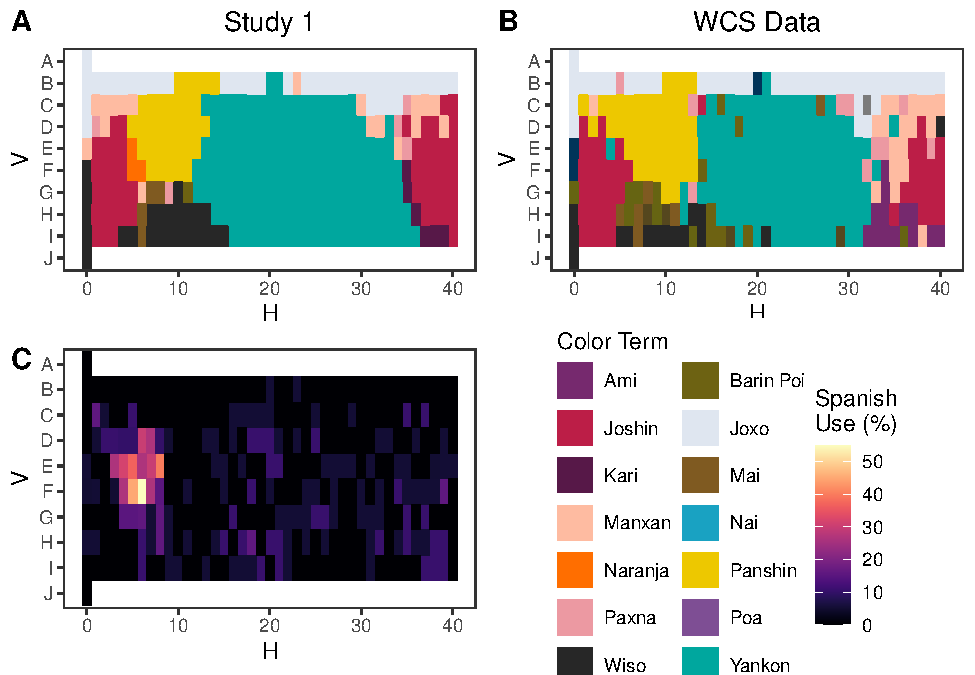
\includegraphics{amazon_color_files/figure-latex/study1-figure-1.pdf}
\caption{\label{fig:study1-figure}(A and B) Plots of the modal term given for a particular chip. Color coordinates were represented in 2-D Munsell space. Modal responses were given by SK adults during (A) the original World Color Survey and during (B) our Study 1. (C) Heat map of prevalence of Spanish-language responses during Study 1. Legends for all three subplots located in the bottom-right quadrant.}
\end{figure}

Participants used an SK-language BCT (i.e., \enquote{yankon}) to describe a median of 65\% of chips (\emph{IQR} = 53-90\%). Besides BCTs, 59\% of participants used SK-language ad hoc hue terms (i.e., \enquote{nai} or sky for blue chips) for an overall median of 6\% of chips (\emph{IQR} = 0-19\%). SK-language terms referring to saturation or luminosity of a chip, such as \enquote{manxan} (faded) were used for an overall median of 13\% of chips (IQR = 6-20\%). Most instances (91\%) of Spanish use involved a Spanish BCT such as \enquote{rojo} (overall \emph{Mdn} = 1\%, \emph{IQR} = 0-4\%). In other words, participants responded in Spanish to label chips with basic color categories but mostly relied on SK for all other descriptor types.

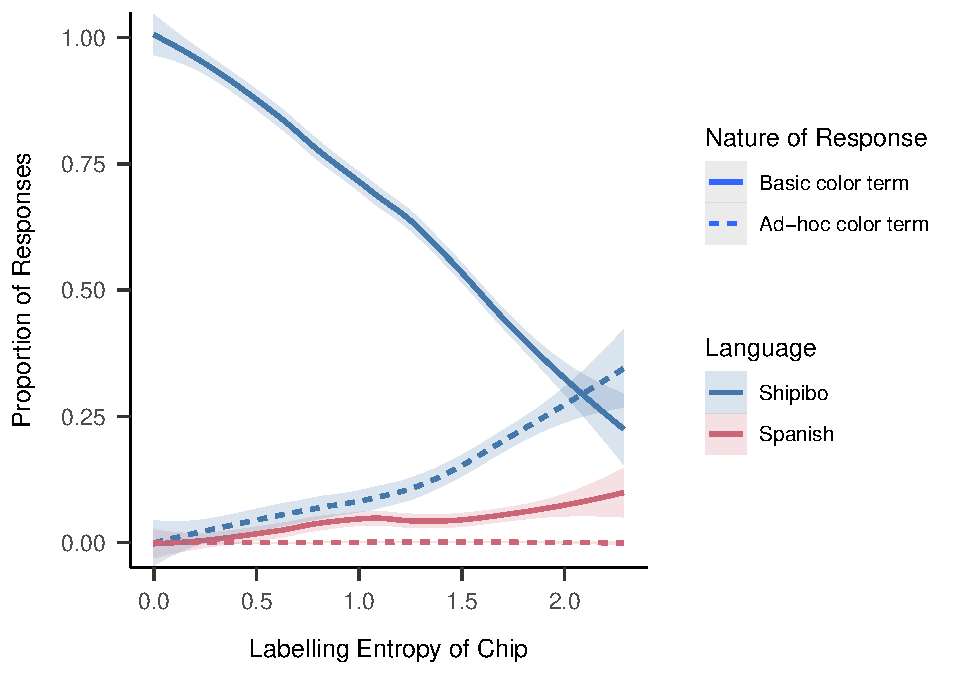
\includegraphics{amazon_color_files/figure-latex/study1-corrected_entropy-1.pdf}

\hypertarget{study-2}{%
\section{Study 2}\label{study-2}}

After generating an updated SK color term map using the responses from adult participants in Study 1, we created Study 2 as a means for assessing child participants' production and comprehension of SK color terms. This study used a subset of chips representing the prototypical instances for prominent SK terms from Study 1.

\hypertarget{methods-1}{%
\subsection{Methods}\label{methods-1}}

\hypertarget{participants-1}{%
\subsubsection{Participants}\label{participants-1}}

\begin{table}[tbp]

\begin{center}
\begin{threeparttable}

\caption{\label{tab:study2-demographics}Demographics of participants in Study 2.}

\begin{tabular}{lll}
\toprule
Age Group & \multicolumn{1}{c}{n} & \multicolumn{1}{c}{Boys}\\
\midrule
5 & 3 (5\% of overall sample) & 1\\
6 & 8 (14\%) & 3\\
7 & 12 (21\%) & 4\\
8 & 15 (26\%) & 5\\
9 & 10 (18\%) & 5\\
10 & 4 (7\%) & 2\\
11 & 5 (9\%) & 3\\
\bottomrule
\end{tabular}

\end{threeparttable}
\end{center}

\end{table}

Fifty-seven children (23 boys) ages 5- to 11-years-old were recruited in predominantly SK neighborhoods in Yarinacocha (Nueva Era and Bena Jema) and in Bawanisho, a native community settled along the Ucayali River, more than 500 kilometers southeast of Pucallpa. Recruitment occurred either through direct contact with interested parents or through their local school. If recruited via school, consent for participation had to be given by both teacher and parent. Outside of the school environment, consent was only given by the parent.

\hypertarget{materials-and-procedure-1}{%
\subsubsection{Materials and procedure}\label{materials-and-procedure-1}}

Based on the findings of Study 1, we chose 8 color chips from our original set of 330 to serve as prototypical instances of major SK color terms. These color chips were blue (WCS n°1), green (n°234), red (n°245), white (n°274), yellow (n°297), black (n°312), greeny-yellow (WCS n°320), and purple (WCS n°325) (see Appendix 1). Study 2 was conducted entirely in SK and participants were explicitly instructed to give responses in SK as opposed to Spanish. In production and comprehension tasks, children sat at a table across from the experimenter with color chips arranged between them. The production task was always performed before the comprehension task.

\hypertarget{procedure}{%
\subsubsection{Procedure}\label{procedure}}

\textbf{Production task.} Similar to Study 1, the experimenter introduced a participant to the general procedure and the goals of the study. The experimenter would then ask: \enquote{What is the color of this chip?}. As in Study 1, we used follow-up questions to elicit a BCT when initial response was not. In a departure from Study 1, we were more explicit in soliciting an SK-language response. When a participant provided a Spanish-language term, the experimenter would record their response but further ask: \enquote{What is the name of this color in SK?}. If a participant could not respond with an SK term, the experimenter would not ask further questions and would move forward to the next chip. As a result, some children could only produce SK non-BCTs or Spanish-language terms for particular chips.

\textbf{Comprehension task.} The comprehension task had a notably different procedure compared to the preceding production task or that of Study 1. The comprehension of 9 SK color terms was tested. The choice of these terms was based on common responses given by adult participants in Study 1. The color term prompts included BCTs: \emph{yankon} (\enquote{green/blue}), \emph{joshin} (\enquote{red}), \emph{panshin} (\enquote{yellow}), \emph{joxo} (\enquote{white/light}), \emph{wiso} (\enquote{black/dark}). We also included non-basic but prominent terms as prompts which were \emph{nai} (\enquote{blue/sky}), and \emph{barin poi} (\enquote{greenish-yellow}) and two dyads of non-basic terms \emph{pei}/\emph{xo} (\enquote{green}) and \emph{ami}/\emph{pua} (\enquote{purple}).

A participant would sit at a table across from the experimenter with 8 color chips of the production task displayed in front. The experimenter would then ask: \enquote{Can you give me the {[}\emph{color term}{]} chip?}. A participant would choose one of the 8 chips and their response recorded. Findings from Study 1 emphasized that color terms varied in their degrees of specificity. For example, \emph{wiso} best describes a narrow range of very dark to black. By contrast, \emph{yankon} could encompass blue, green, greenish-yellow, and purple; \emph{joshin} could describe red, purple, and orange; \emph{pei} or \emph{xo} to green or greenish-yellow.

In cases where a term could apply for more than one chip (i.e., \emph{yankon}), the initially selected chip would be removed from the table, leaving 7 remaining chips. The experimenter would then ask: \enquote{Can you give me another {[}\emph{color term}{]} chip?}. A participant would pick another one of the 7 chips, have their response recorded, and so on. A participant would be prompted 4 times for \emph{yankon} and 2 times each for \emph{joshin} and \emph{pei}/\emph{xo}, every other term only received a single prompt. Due to the inherent ambiguity in term-hue pairings, accuracy for a child participant was coded based on adult responses given during Study 1. If at least 15\% of adult participants in Study 1 associated a chip with a particular term, we coded a similar term-chip pairing from a child participant as correct. Unlike the production task, as some trials could have multiple pairings, accuracy was scored as an average, rather than dichotomous. For instance, if a child correctly chose 3 out of 4 chips for the \enquote{yankon} trial, instead of 1 (correct) or 0 (incorrect) they would receive a score of 0.75.

\begin{figure}
\centering
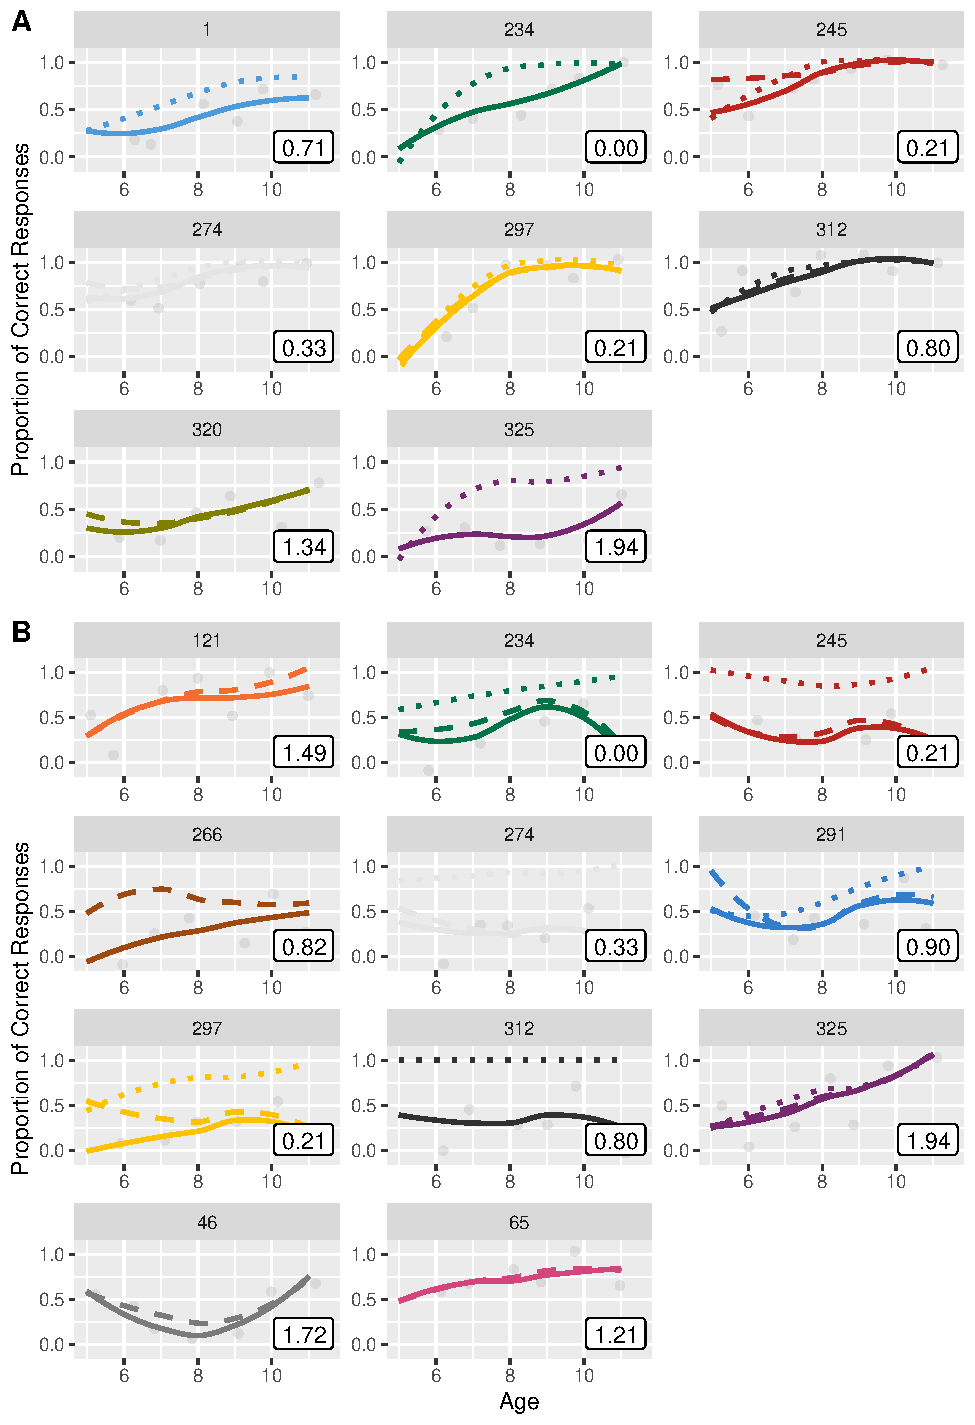
\includegraphics{amazon_color_files/figure-latex/prod-childfigure-1.pdf}
\caption{\label{fig:prod-childfigure}(A and B) A comparison of children's performance during the production task in Studies 2 (top) and 3 (bottom). Solid or dotted lines represent overall performance by age for a particular chip. Solid lines show whether the child gave a correct answer in the language indicated in that column; dotted lines show if they gave a response that was correct in either language. Line colors are representative of the chip's color coordinates.}
\end{figure}

\begin{table}[tbp]

\begin{center}
\begin{threeparttable}

\caption{\label{tab:study2-prodtable}Demographics of participants in Study 2.}

\begin{tabular}{llllllll}
\toprule
prompt & \multicolumn{1}{c}{5-years-old (3 children)} & \multicolumn{1}{c}{6-years-old (8)} & \multicolumn{1}{c}{7-years-old (12)} & \multicolumn{1}{c}{8-years-old (15)} & \multicolumn{1}{c}{9-years-old (10)} & \multicolumn{1}{c}{10-years-old (4)} & \multicolumn{1}{c}{11-years-old (5)}\\
\midrule
n°1 (Celeste) & 0.33 & 0.25 & 0.17 & 0.53 & 0.40 & 0.75 & 0.60\\
n°234 (Verde) & 0.00 & 0.38 & 0.50 & 0.53 & 0.70 & 0.75 & 1.00\\
n°245 (Rojo) & 0.67 & 0.38 & 0.75 & 0.87 & 1.00 & 1.00 & 1.00\\
n°274 (Blanco) & 0.67 & 0.62 & 0.58 & 0.87 & 1.00 & 0.75 & 1.00\\
n°297 (Amarillo) & 0.00 & 0.25 & 0.58 & 0.93 & 0.90 & 0.75 & 1.00\\
n°312 (Negro) & 0.33 & 0.88 & 0.58 & 1.00 & 1.00 & 1.00 & 1.00\\
n°320 (Mierda sol) & 0.33 & 0.25 & 0.25 & 0.40 & 0.60 & 0.25 & 0.80\\
n°325 (Morado) & 0.00 & 0.25 & 0.25 & 0.20 & 0.20 & 0.25 & 0.60\\
Overall & 0.29 & 0.41 & 0.46 & 0.67 & 0.72 & 0.69 & 0.88\\
\bottomrule
\end{tabular}

\end{threeparttable}
\end{center}

\end{table}

\begin{table}[tbp]

\begin{center}
\begin{threeparttable}

\caption{\label{tab:study2-accuracyswitchentropy}}

\begin{tabular}{lllll}
\toprule
Term & \multicolumn{1}{c}{$\hat{\beta}$} & \multicolumn{1}{c}{95\% CI} & \multicolumn{1}{c}{$z$} & \multicolumn{1}{c}{$p$}\\
\midrule
Intercept & -2.87 & [-3.70, -2.05] & -6.85 & < .001\\
Age years c & -0.52 & [-1.01, -0.03] & -2.09 & .036\\
Entropy & 1.54 & [1.02, 2.06] & 5.82 & < .001\\
Entropy & 0.34 & [0.03, 0.66] & 2.13 & .034\\
\bottomrule
\end{tabular}

\end{threeparttable}
\end{center}

\end{table}

\begin{figure}
\centering
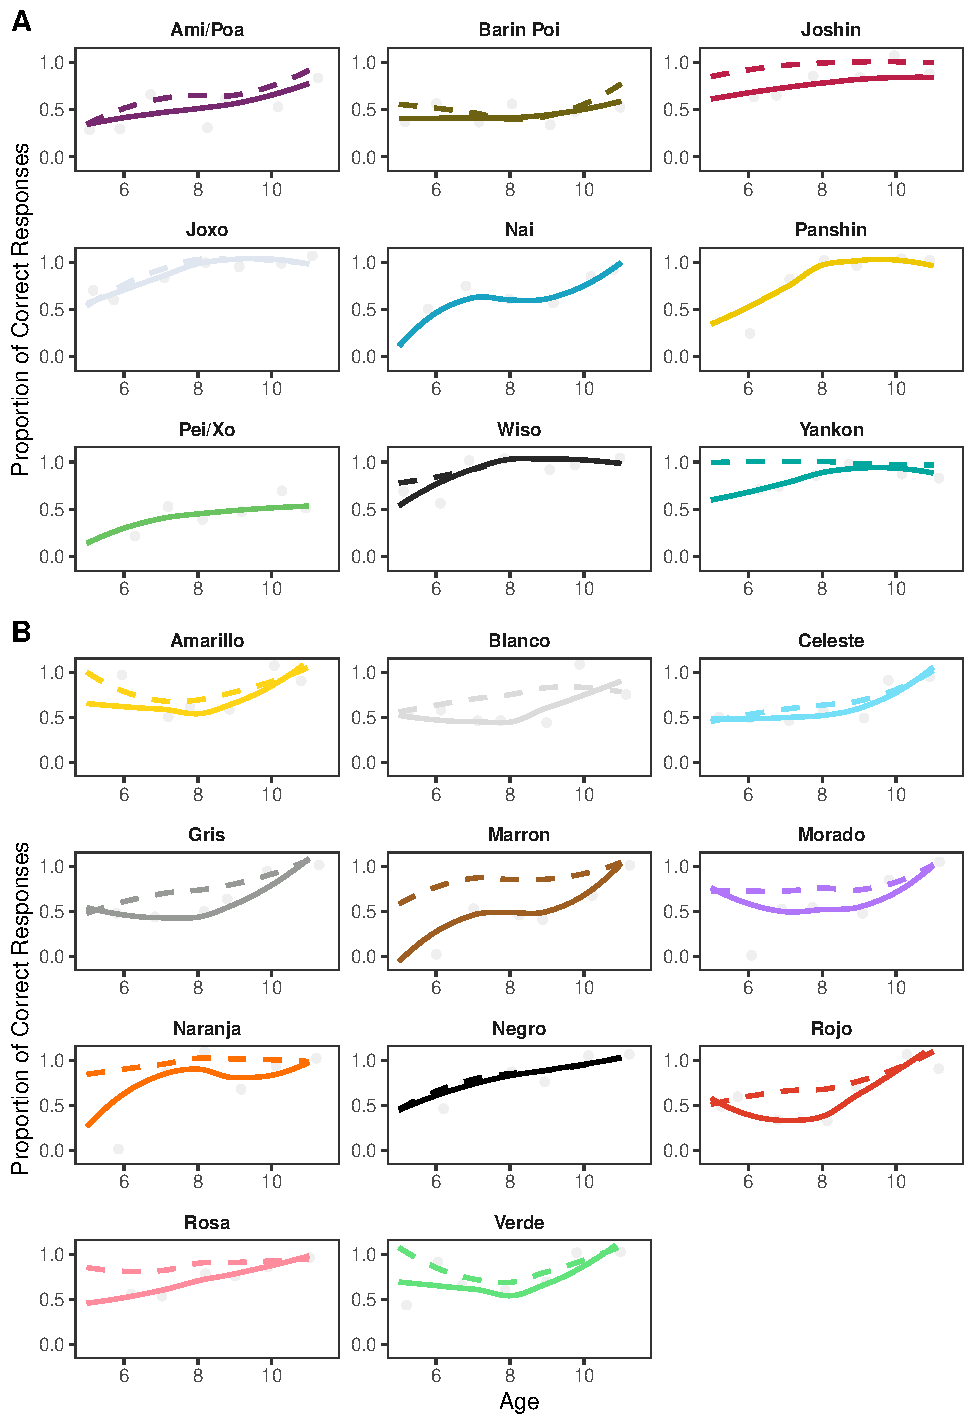
\includegraphics{amazon_color_files/figure-latex/comp-childfigure-1.pdf}
\caption{\label{fig:comp-childfigure}(A and B) A comparison of children's performance during the comprehension tasks in Studies 2 (top) and 3 (bottom). Solid or dotted lines represent overall performance by age for a particular chip. Solid lines show whether the child chose the correct chip when prompted with a color term; dotted lines show whether a child chose the correct chip or a chip from an adjacent color category. Line colors are representative of the label's prototypical color coordinates.}
\end{figure}

\begin{figure}
\centering
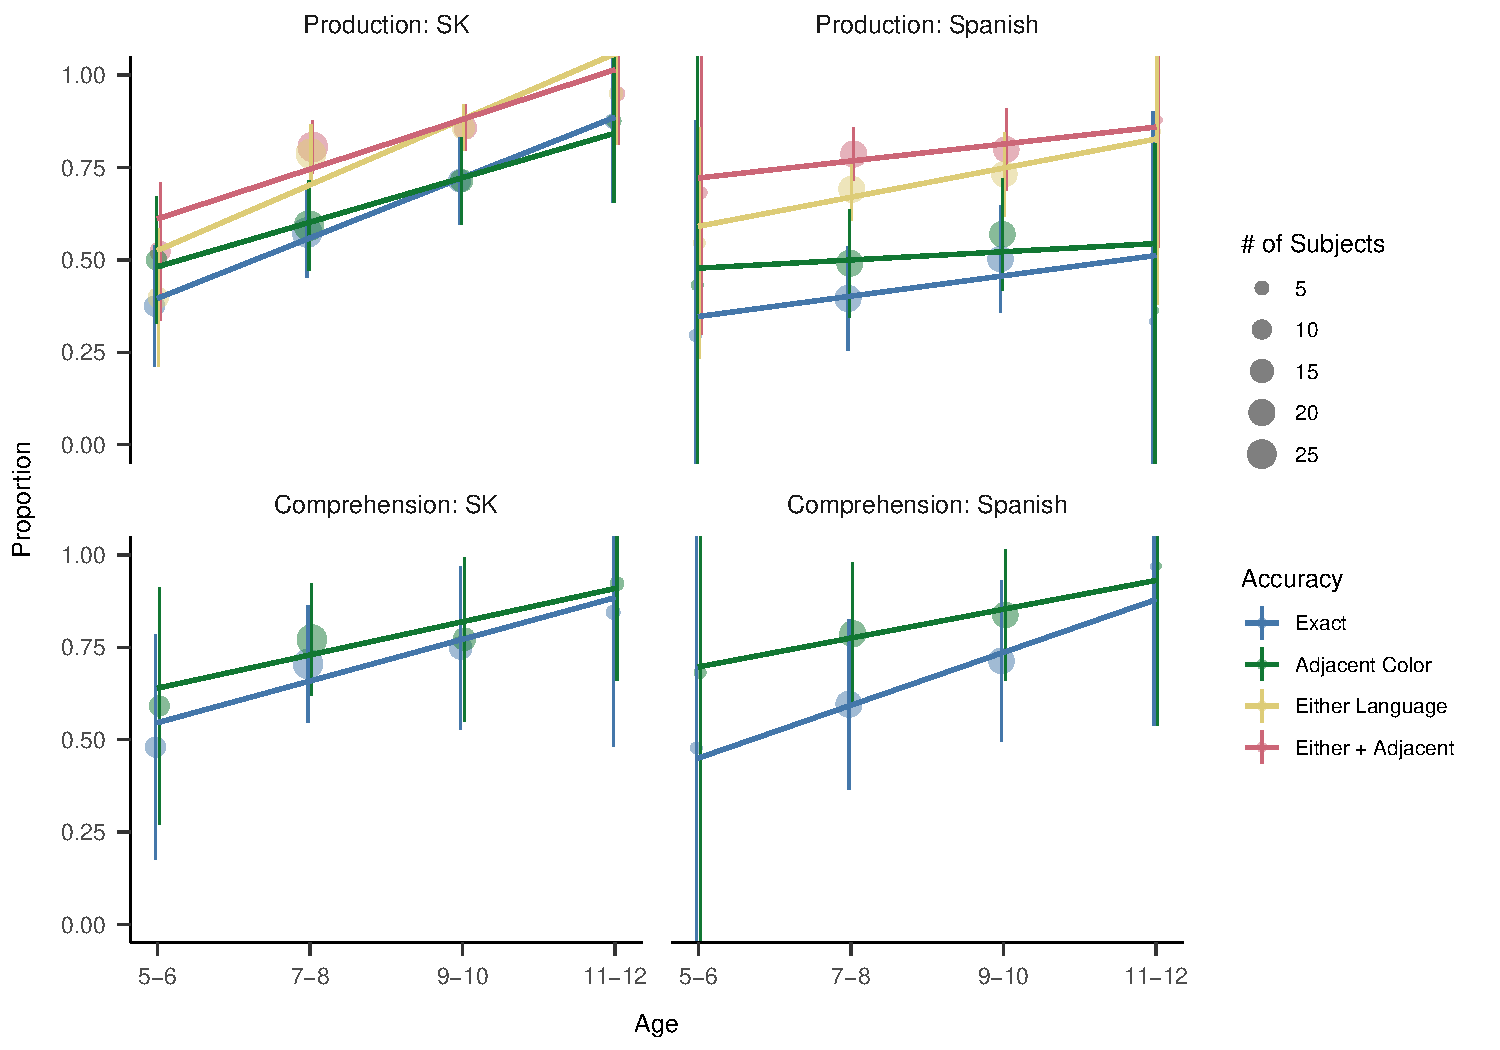
\includegraphics{amazon_color_files/figure-latex/study23-accuracy-1.pdf}
\caption{\label{fig:study23-accuracy}Proportion of accurate responses when applying different accuracy criteria, by age and study. Points show the mean for a 2-year age group (chosen arbitrarily for visualization) with 95\% confidence intervals. Lines show a loess smoothing function. Points show the mean for a 2-year age group (chosen arbitrarily for visualization) with 95\% confidence intervals.}
\end{figure}

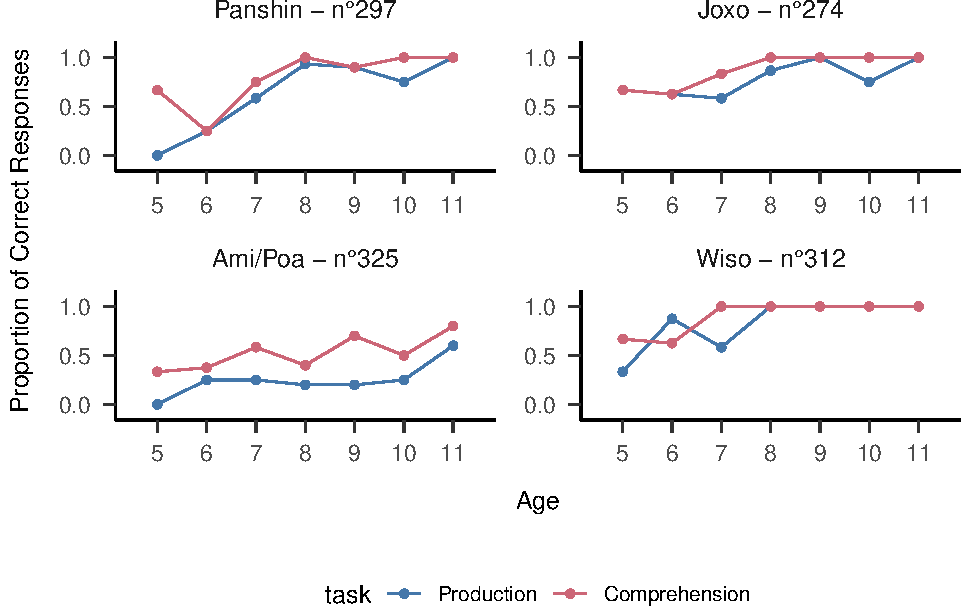
\includegraphics{amazon_color_files/figure-latex/study2-task-compare-plot-1.pdf}

\hypertarget{results-and-discussion-1}{%
\subsection{Results and Discussion}\label{results-and-discussion-1}}

Older children were more accurate in both production and comprehension compared to younger children (Figure \ref{fig:study23-accuracy}). This produced a significant developmental projection for accuracy of term-chip pairings in both production (\(z = 3.74\), \(p < .001\)) and comprehension (\(z = 3.27\), \(p = .001\)). For some term-chip pairings such as ami/pua and pei/xo, children performed failed to produce the correct term in the production task but improved significantly during the comprehension task (Figure \ref{fig:study2-task-compare-plot}). It is possible that for children's color term knowledge, comprehension precedes production. It is also possible that, given that the comprehension task always followed the production task, children were able to pick up on their errors and update their color term mapping in real-time. However, given that the experimenter did not provide feedback on accuracy during sessions, the former explanation seems more likely.

\textbf{Language switching.} Over a quarter (28\%) of all responses were given in Spanish, despite children being prompted solely in SK (i.e., labeling a panshin chip as \enquote{amarillo}). The distribution of Spanish responses was non-random, with median use in 2/8 trials (IQR = 0-5). We failed to find a significant correlation between age and overall Spanish use throughout the production task (\(t(55) = -1.13\), \(p = .263\)).

As an exploratory analysis, we attempted to quantify low naming consensus using naming entropy (following Gibson et al., 2017). We computed the naming entropy for each chip by computing the probabilities for each chip \(c\) to be named with a particular label \(l\) (\(p(l \mid c)\)) and then taking \(H(c) = - \sum{p(l\mid c) \log[p(l \mid c)]}\) (see inset entropy values by chip in Figure \ref{fig:prod-childfigure}).
To assess the hypothesis that naming entropy in adults was related to Spanish use in children, we fit a mixed effects model predicting Spanish responses as a function of child age, entropy of the chip's naming distribution for adults in Study 1, and their interaction. Despite age not being significantly correlated with overall frequency of Spanish responses, when added to a mixed-effects model, we found that older children were less likely to respond in Spanish (Table \ref{tab:study2-accuracyswitchentropy}). Older children were also more likely to respond in Spanish when presented with a chip with high entropy (low naming consensus) among adult participants in Study 1. We found a positive interaction between age and entropy.

\textbf{Overextensions.}

One reason to use Spanish would be if children fail to recall the proper SK color term but do know the proper mapping in the Spanish. But another possibility is that children may have more imprecise representations and choose to respond with a same-language but adjacent color term (i.e., labeling a \emph{panshin}-colored chip as \enquote{joshin}). Following Wagner et al. (2013), we aggregated across color chips and examine the pattern of children's first responses, categorizing them as same-language, adjacent, and different-language. Using a mixed-effects model, we found that younger children were more likely to respond with SK-language but adjacent terms (\(\hat{\beta} = -1.16\), 95\% CI \([-1.96, -0.35]\)) but chip entropy did not have a significant factor in this strategy (\(\hat{\beta} = -1.23\), 95\% CI \([-3.00, 0.54]\)).

If children fail to recall the proper color term in SK, but do know the proper mapping in the Spanish color system, language-switching may be an appropriate strategy. Should they lack knowledge of the corresponding Spanish color term, they may also choose to respond with a same-language but adjacent color term. If we allow for more leniency in scoring--accepting same-language but adjacent or different-language but corresponding responses--we can check for more subtlety surrounding color term mapping (Figure \ref{fig:study23-accuracy}). Using a mixed-effects model, we found a significant improvement in accuracy scores when we allowed different-language but corresponding responses (\(z = 6.98\), \(p < .001\)) but no significant change when allowing for same-language but adjacent responses (\(z = 0.86\), \(p = .390\)). This increase in accuracy with language-switching strengthened with age (\(z = 2.74\), \(p = .006\)).

\hypertarget{study-3}{%
\section{Study 3}\label{study-3}}

Noting the apparent strategy of language switching seen in Study 2, we designed Study 3 as its complement. Here, we tested children's production and comprehension of Spanish color terms with a similar protocol to Study 2 albeit with a subset of chips representing prototypical colors for the Spanish color system.

\hypertarget{participants-2}{%
\subsubsection{Participants}\label{participants-2}}

\begin{table}[tbp]

\begin{center}
\begin{threeparttable}

\caption{\label{tab:study3-demographics}Demographics of participants in Study 3.}

\begin{tabular}{lll}
\toprule
Age Group & \multicolumn{1}{c}{n} & \multicolumn{1}{c}{Boys}\\
\midrule
5 & 2 (4\% of overall sample) & 1\\
6 & 2 (4\%) & 0\\
7 & 11 (24\%) & 4\\
8 & 9 (20\%) & 1\\
9 & 11 (24\%) & 4\\
10 & 8 (17\%) & 3\\
11 & 3 (7\%) & 3\\
\bottomrule
\end{tabular}

\end{threeparttable}
\end{center}

\end{table}

Similar to Study 2, 46 children (16 boys) ages 5- to 11-years-old were recruited from the neighborhood of Bena Jema in Yarinacocha and from Bawanisho. Recruitment occurred either through interested parents or a local school. With consent collected from parents and, if in a school environment, teachers as well.

\hypertarget{materials-and-procedure-2}{%
\subsubsection{Materials and procedure}\label{materials-and-procedure-2}}

Based on Study 1 and on previous studies of Spanish color systems (XXX et al), we selected 11 color chips to serve as prototypical instances of prominent Peruvian Spanish color terms. These color chips included 6 also used during Study 2: green (n°234), red (n°245), white (n°274), yellow (n°297), black (n°312) , and purple (n°325). Five additional chips were selected: gray (WCS n°46), pink (n°65), orange (n°121), brown (n°266), and blue (n°291) (see Appendix 1). It should be noted that the blue chips differed between both Studies 2 and 3 as we decided that the prototypical hues for \emph{yankon} and \emph{azul} differed enough to warrant a different chip.

As SK children are not very fluent in Spanish (formal Spanish education occurs in adolescence), the production and comprehension tasks were both conducted in SK, and Spanish was only used for color terms (i.e., Spanish color terms were embedded within otherwise SK sentences). In both tasks, a participant would sit at a table across from the experimenter with 11 color chips in front. As in Study 2, the production task was always performed prior to the comprehension task.

\textbf{Production task}. The procedure was similar to that of both Studies 1 and 2. The experimenter would introduce a participant to the general procedure and aims of the study. Despite much of the study being conducted in SK, the experimenter would specify that participants would be expected to provide color terms in Spanish. The experimenter would then ask: \enquote{What is the color of this chip?}. If the participant responded in SK, the experimenter would record their response but further ask: \enquote{What is the name of this color in Spanish?}. If a participant responded with \enquote{I don't know} to this prompt, the experimenter would not prompt any further and would move forward to the next chip. As a result, some responses lack Spanish-language BCTs and only consist of non-basic and/or SK color terms. In total, we collected production data for 11 color chips. For each chip, the data include either one response when children provided a Spanish basic color term in the first trial or 2-3 responses when children's initial responses were either non-basic and/or in SK.

\textbf{Comprehension task.} The procedure was similar to that of Study 2. The experimenter would ask: Can you give me the {[}color term{]} chip? For 11 Spanish color terms. The choice of these terms was based on both previous studies examining Spanish color terms as well as responses given by adult participants in Study 1 (as some adult participants used Spanish color terms to label particular color chips). The 11 terms used as prompts were \emph{blanco} (\enquote{white}), \emph{verde} (\enquote{green}), \emph{rojo} (\enquote{red}), \emph{amarillo} (\enquote{yellow}), \emph{azul} (\enquote{blue}), \emph{negro} (\enquote{black}), \emph{naranja} (\enquote{orange}), \emph{gris} (\enquote{grey}), \emph{morado} (\enquote{purple}), \emph{marrón} (\enquote{brown}), and \emph{rosa} (\enquote{pink}). Since each color term was best instantiated by a single color chip and lacked the ambiguity seen with certain SK color terms, accuracy was graded one-to-one for term-chip pairings with less leniency compared to Study 2.

\begin{table}[tbp]

\begin{center}
\begin{threeparttable}

\caption{\label{tab:study3-accuracyswitchentropy}}

\begin{tabular}{lllll}
\toprule
Term & \multicolumn{1}{c}{$\hat{\beta}$} & \multicolumn{1}{c}{95\% CI} & \multicolumn{1}{c}{$z$} & \multicolumn{1}{c}{$p$}\\
\midrule
Intercept & 0.67 & [-0.12, 1.46] & 1.67 & .095\\
Age years c & -0.02 & [-0.49, 0.45] & -0.08 & .939\\
Entropy & -1.49 & [-2.07, -0.92] & -5.10 & < .001\\
\bottomrule
\end{tabular}

\end{threeparttable}
\end{center}

\end{table}

\hypertarget{results-and-discussion-2}{%
\subsection{Results and Discussion}\label{results-and-discussion-2}}

Contrasting Study 2, we found age to be a significant predictor of accuracy in the comprehension task (\(z = 2.90\), \(p = .004\)), but not in the production task (\(z = 1.61\), \(p = .108\), see Figure \ref{fig:study23-accuracy}). Similar to Study 2, over a quarter (30\%) of all responses were given in SK, despite being prompted to respond in Spanish. There was significant variation in language-switching with some children responding solely in Spanish while others responded to upwards of 9/11 trials in SK (Mdn = 5 trials, IQR = 1.25-6). We found only a marginal correlation between age and label accuracy (\(t(44) = 1.91\), \(p = .063\)) and an insignificant correlation between age and language-switching (\(t(44) = 0.44\), \(p = .663\)). Still, when accounting for age, we found that participants tended to respond in SK when presented with items that had low entropy in Study 1 (\(z = -5.10\), \(p < .001\)). This suggests that child participants across Studies 2 and 3 preferred to respond in SK when presented with a high-consensus chip, and in Spanish with a low-consensus chip.

Similar to Study 2, we adopted alternative scoring to accommodate language-switching from Spanish to SK (different-language) but corresponding and same-language but adjacent responses. Using a mixed-effects model, we failed to find age as a significant predictor for accuracy even with this more lenient scoring (\(z = 1.45\), \(p = .146\)), in concordance with earlier analyses. However, we did find that participants improved accuracy through both mapping strategies of either providing different-language but corresponding responses (\(z = 10.51\), \(p < .001\)) or same-language but adjacent responses (\(z = 3.29\), \(p = .001\)). We find frequent use of language switching in both Studies 2 and 3, but only Study 3 exhibits significant use of same-language but adjacent terms.

It is possible that early but informal Spanish language exposure can explain the discrepancies seen in Studies 2 and 3. Children may be exposed to Spanish at a young age but likely do not receive any formal Spanish education until adolescence. With limited knowledge of Spanish color terms, children may spontaneously supplement their color term knowledge with Spanish terms during SK-language Study 2 but struggle to succeed during Spanish-language Study 3. More generally, we see children relying on a mixture of strategies to communicate colors even in the absence of mastery in either language.

\hypertarget{general-discussion}{%
\section{General Discussion}\label{general-discussion}}

TO BE PASTED FROM GOOGLE DOC

Summary of study.
Adult data - bilingualism and relation to WCS data
When we turned to the children's data, two important generalizations emerged. First, we observed a much longer developmental trajectory for color than is observed in modern US populations (cf.~Bornstein, 1985).
Second, we found evidence for competition between the Shipibo and Spanish color systems, implying the potential for functionally-driven language change.
Gibson analysis of optimality: children use spanish words for low-consensus chips, SK words for high consensus chips. These support the optimality hypothesis
Limitations of our work.
Cross-sectional
Limited number of chips for kids (limits entropy analyses)

In sum, these data further support a model of color word knowledge and acquisition that is driven by communicative need.
Need for more developmental work on other languages.
Huge role for environmental input

\newpage

\hypertarget{references}{%
\section{References}\label{references}}

\begingroup
\setlength{\parindent}{-0.5in}
\setlength{\leftskip}{0.5in}

\hypertarget{refs}{}
\leavevmode\hypertarget{ref-apicella2016}{}%
Apicella, C. L., \& Barrett, H. C. (2016). Cross-cultural evolutionary psychology. \emph{Current Opinion in Psychology}, \emph{7}, 92--97.

\leavevmode\hypertarget{ref-aragon2016}{}%
Aragón, K. (2016). Color language and color categorization. In G. Paulsen, M. Uusküla, \& J. Brindle (Eds.). Cambridge Scholars.

\leavevmode\hypertarget{ref-berlin1969}{}%
Berlin, B., \& Kay, P. (1969). \emph{Basic color terms: Their universality and evolution}. Berkeley, CA: University of California Press.

\leavevmode\hypertarget{ref-everett2005}{}%
Everett, D. L. (2005). Cultural constraints on grammar and cognition in pirahã another look at the design features of human language. \emph{Current Anthropology}, \emph{46}(4), 621--646.

\leavevmode\hypertarget{ref-gibson2017}{}%
Gibson, E., Futrell, R., Jara-Ettinger, J., Mahowald, K., Bergen, L., Ratnasingam, S., \ldots{} Conway, B. (2017). Color naming across languages reflects color use. \emph{Proceedings of the National Academy of Sciences}, \emph{114}(40), 10785--10790.

\leavevmode\hypertarget{ref-berlin2009}{}%
Kay, P., Berlin, B., Maffin, L., Merrifield, W. R., \& Cook, R. (2009). \emph{The world color survey}. Stanford, CA: Center for the Study of Language; Information.

\leavevmode\hypertarget{ref-kitayama2007}{}%
Kitayama, S., \& Cohen, D. (2007). \emph{Handbook of cultural psychology}. Guilford Press.

\leavevmode\hypertarget{ref-lathrap1970}{}%
Lathrap, D. W. (1970). \emph{The upper amazon}. Thames; Hudson.

\leavevmode\hypertarget{ref-monroy1989}{}%
Monroy, M., \& Custodio, S. (1989). Algunos usos de los términos del color en el español de colombia. \emph{Thesaurus; Bogotà}, \emph{44}(2), 441.

\leavevmode\hypertarget{ref-morin1973}{}%
Morin, E. (1973). \emph{Le paradigme perdu: La nature humaine}. Éditions du Seuil.

\leavevmode\hypertarget{ref-regier2007}{}%
Regier, T., Kay, P., \& Khetarpal, N. (2007). Color naming reflects optimal partitions of color space. \emph{Proceedings of the National Academy of Sciences}, \emph{104}(4), 1436--1441.

\leavevmode\hypertarget{ref-surralles2016}{}%
Surrallés, A. (2016). On contrastive perception and ineffability: Assessing sensory experience without colour terms in an amazonian society. \emph{Journal of the Royal Anthropological Institute}, \emph{22}(4), 962--979.

\leavevmode\hypertarget{ref-tournon2002}{}%
Tournon, J. (2002). \emph{La merma magica: Vida e historia de los shipibo-conibo del ucayali}. Centro Amazonico de Antropologia Yaplicacion.

\leavevmode\hypertarget{ref-wagner2013}{}%
Wagner, K., Dobkins, K., \& Barner, D. (2013). Slow mapping: Color word learning as a gradual inductive process. \emph{Cognition}, \emph{127}, 307--317.

\endgroup


\end{document}
